\section{Programos kodas}
\label{sec:programos_kodas}

Šiame skyriuje pateikiami svarbiausių klasių kodo fragmentai su komentarais. Kodo struktūra suskaidyta į modulius pagal atsakomybę:
\begin{itemize}
    \item \texttt{DataSplitter/} – pradinio duomenų rinkinio padalijimas į \textit{train}, \textit{validation} ir \textit{test} aibes.
    \item \texttt{DataReader/} – paruoštų aibių užkrovimas į \texttt{torch} duomenų objektus.
    \item \texttt{Models/} – konvoliucinių neuroninių tinklų architektūros (\texttt{BaseCNN}, \texttt{ImageCNN}, \texttt{KeystrokeCNN}).
    \item \texttt{Utils/} – pagalbinės klasės (\texttt{Trainer}, \texttt{KeystrokeDataset}, \texttt{get\_device}).
    \item \texttt{Enums/} – enumeracijos su palaikomais aktyvavimo, optimizavimo ir nuostolių algoritmais.
    \item \texttt{main.py} – eksperimentų vykdymas ir geriausio modelio įvertinimas.
\end{itemize}

\subsection{Vaizdų duomenų skaitytuvo klasė}
\label{subsec:image_data_reader}

Klasė \texttt{ImageDataReader} užkrauna jau padalintas vaizdų aibes ir pritaiko vienodą \texttt{torchvision.transforms} grandinę. Skaičiavimo resursams taupyti buvo užkraunama $30\ \%$ duomenų (žr.~\ref{fig:image_data_reader_class} pav.).

\begin{figure}[H]
    \centering
    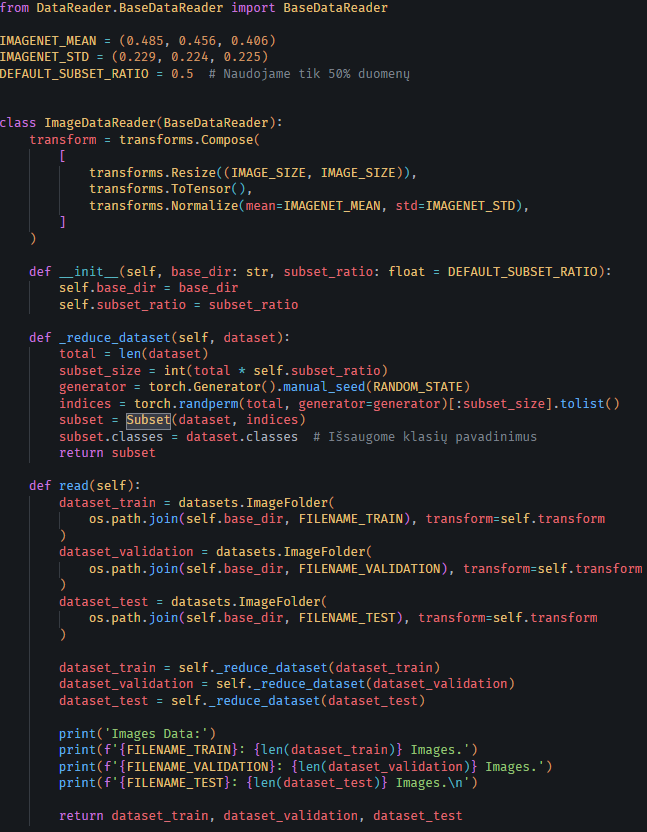
\includegraphics[width=0.85\linewidth]{3Lab/overleaf/images/ImageDataReader_Class.png}
    \caption{Vaizdų duomenų skaitytuvo klasės kodas.}
    \label{fig:image_data_reader_class}
\end{figure}

Klasės veikimo žingsniai:
\begin{enumerate}
    \item \texttt{transforms.Resize} suvienodina visus vaizdus į $64 \times 64$ raišką – tinklo įėjimo formatas turi būti pastovus.
    \item \texttt{transforms.ToTensor} konvertuoja \texttt{PIL.Image} į \texttt{torch.Tensor} ir pikselius perkelia į $[0,\,1]$ intervalą.
    \item \texttt{transforms.Normalize} standartizuoja kanalus pagal \textit{ImageNet} vidurkį ir standartinį nuokrypį, todėl tinklo svoriai pradeda mokytis stabilesnėje skaitinėje erdvėje.
    \item \texttt{\_reduce\_dataset} atsitiktinai parenka \texttt{subset\_ratio} dalį indeksų ir grąžina \texttt{torch.utils.data.Subset}. Naudojamas atskiras \texttt{torch.Generator} su \texttt{seed = 42}, todėl pošalis kiekvieną kartą yra tas pats.
    \item \texttt{read} paima visus tris \texttt{ImageFolder} aplankus (\textit{train}, \textit{validation}, \textit{test}) ir grąžina jų sumažintus pošalius.
\end{enumerate}

Klasės kodas parašytas autoriaus, naudojantis oficialia \texttt{torchvision} dokumentacija. \textit{ImageNet} statistikos reikšmės paimtos iš \texttt{torchvision} oficialaus pavyzdžio kodo.

\subsection{Laiko eilučių duomenų dalijimo klasė}
\label{subsec:keystroke_data_splitter}

Klasė \texttt{KeystrokeDataSplitter} iš pradinio CMU CSV failo paruošia \textit{train}, \textit{validation} ir \textit{test} aibes: pasirenka subjektus, normalizuoja požymius ir stratifikuotai padalija duomenis (žr.~\ref{fig:keystroke_data_splitter_class_first} ir \ref{fig:keystroke_data_splitter_class_last} pav.).

\begin{figure}[H]
    \centering
    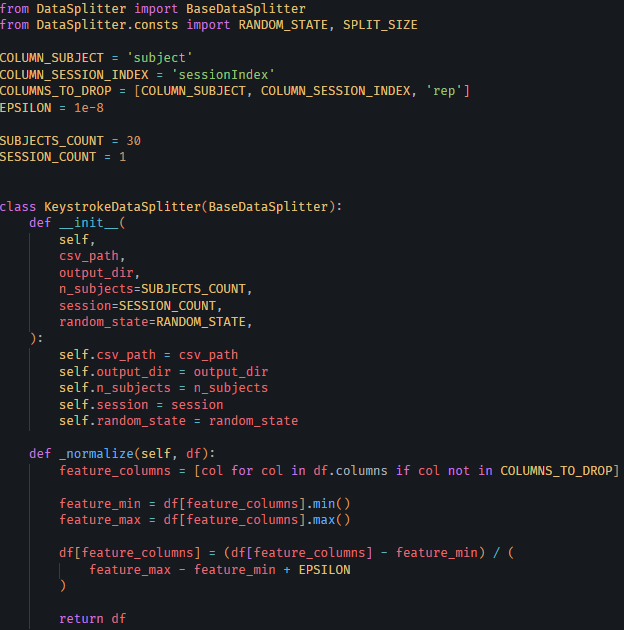
\includegraphics[width=0.85\linewidth]{3Lab/overleaf/images/KeystrokeDataSplitter_Class_1.png}
    \caption{Laiko eilučių duomenų dalijimo klasės kodas I dalis.}
    \label{fig:keystroke_data_splitter_class_first}
\end{figure}

\begin{figure}[H]
    \centering
    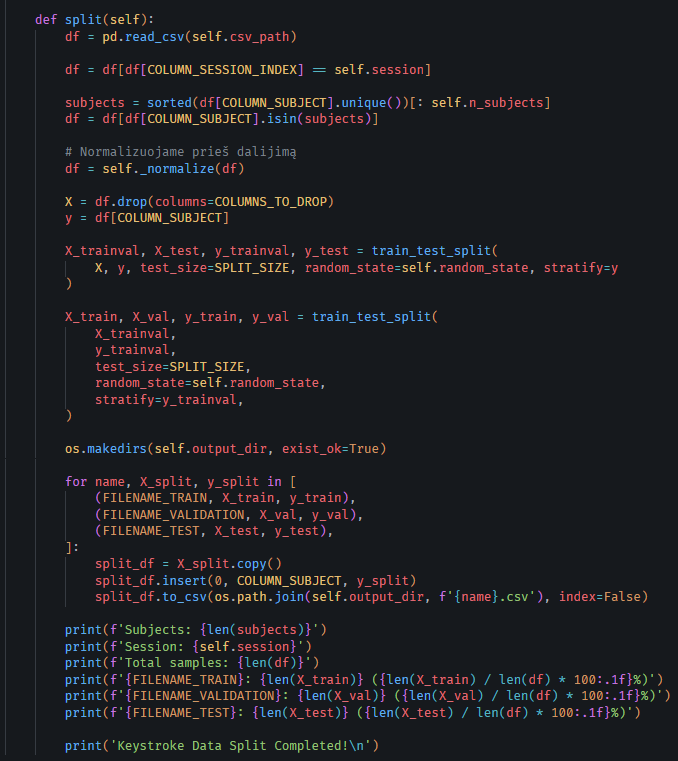
\includegraphics[width=0.85\linewidth]{3Lab/overleaf/images/KeystrokeDataSplitter_Class_2.png}
    \caption{Laiko eilučių duomenų dalijimo klasės kodas II dalis.}
    \label{fig:keystroke_data_splitter_class_last}
\end{figure}

Klasės veikimo žingsniai:
\begin{enumerate}
    \item Iš pradinio CSV nuskaitomos $20\,400$ eilučių; paliekama tik viena sesija (\texttt{sessionIndex}~$=1$).
    \item Iš likusių dalyvių abėcėline tvarka atrenkami pirmieji $30$ subjektai – gauname $30$ klasių klasifikavimo užduotį su $1\,500$ įrašų.
    \item Visi $31$ laikinis požymis normalizuojami min-max metodu į $[0,\,1]$. \texttt{EPSILON}~$=10^{-8}$ apsaugo nuo dalybos iš nulio, jei stulpelio reikšmės sutampa.
    \item Atliekamas dvigubas stratifikuotas dalijimas (\texttt{stratify=y}): pirmas – $80\,\%$ \textit{train+val} ir $20\,\%$ \textit{test}; antras – iš \textit{train+val} aibės dar $80\,\%$ / $20\,\%$ į \textit{train} ir \textit{validation}. Bendras santykis – $64{:}16{:}20$.
    \item Trys gautos aibės įrašomos į atskirus CSV failus, iš kurių vėliau \texttt{KeystrokeDataReader} užkrauna duomenis į \texttt{KeystrokeDataset}.
\end{enumerate}

Klasės kodas parašytas autoriaus. \texttt{sklearn.model\_selection.train\_test\_split} idioma su \texttt{stratify=y} paimta iš \texttt{scikit-learn} oficialios dokumentacijos. Min-max formulę su $\varepsilon$ apsauga padėjo suformuluoti Claude.

\subsection{Bazinė CNN modelio klasė}
\label{subsec:base_cnn}

Klasė \texttt{BaseCNN} aprašo bendrą konvoliucinio tinklo šabloną – iš jos paveldi \texttt{ImageCNN} (su \texttt{nn.Conv2d}) ir \texttt{KeystrokeCNN} (su \texttt{nn.Conv1d}). Paveldinčios klasės nurodo tik konvoliucinių, telkimo ir paketinio normalizavimo sluoksnių dimensijas (žr.~\ref{fig:base_cnn_class} pav.).

\begin{figure}[H]
    \centering
    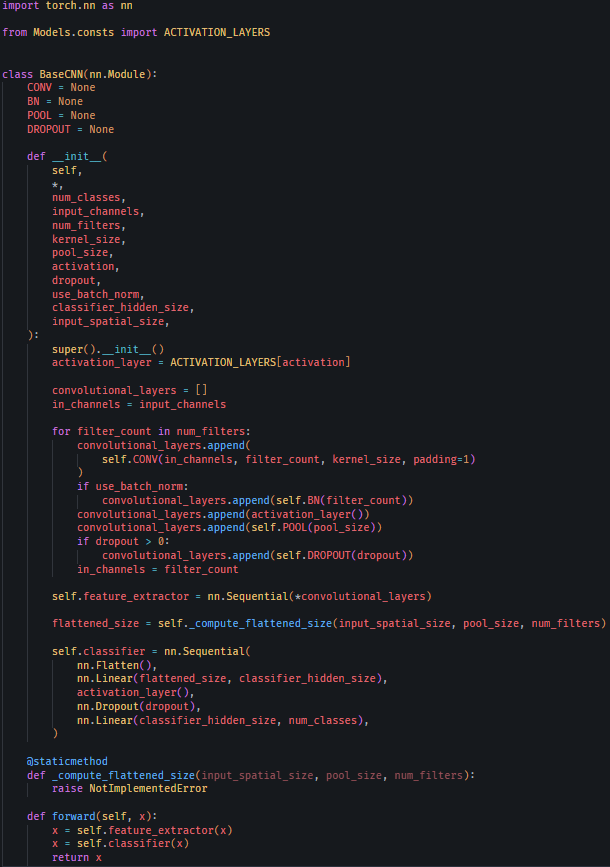
\includegraphics[width=0.85\linewidth]{3Lab/overleaf/images/BaseCNN_Class.png}
    \caption{Bazinės CNN modelio klasės kodas.}
    \label{fig:base_cnn_class}
\end{figure}

Tinklo struktūros komponentai:
\begin{itemize}
    \item \textbf{Konvoliucinis sluoksnis} (\texttt{CONV}) – išmoksta lokalius požymius (briaunos, formos vaizdams; laikinės šablonų formos požymiai laiko eilutėms). \texttt{padding}~$=1$ išlaiko erdvinę dimensiją iki telkimo.
    \item \textbf{Paketinis normalizavimas} (\texttt{BN}) – stabilizuoja tarpinių aktyvavimų pasiskirstymą, leidžia naudoti didesnį mokymosi greitį ir veikia kaip silpnas reguliarizatorius.
    \item \textbf{Aktyvacijos funkcija} – įveda netiesiškumą; konfigūruojama per \texttt{ActivationFunction} enumeraciją (\textit{ReLU}, \textit{LeakyReLU}, \textit{Tanh}, \textit{ELU}, \textit{Sigmoid}).
    \item \textbf{Telkimo sluoksnis} (\texttt{POOL}) – sumažina erdvinę dimensiją perpus, taip didindamas receptyvinį lauką ir mažindamas skaičiavimo kaštus.
    \item \textbf{\textit{Dropout}} – atsitiktinai išjungia dalį neuronų, kovoja su persimokymu (\textit{overfitting}).
    \item \textbf{Klasifikatorius} – \texttt{Flatten}~$\rightarrow$ paslėptas pilnai sujungtas sluoksnis su aktyvacija ir \textit{Dropout}~$\rightarrow$ išėjimo sluoksnis su tiek neuronų, kiek yra klasių (raw \textit{logits}, \texttt{Softmax} įjungiamas \texttt{CrossEntropyLoss} viduje).
\end{itemize}

Mokymo eiga:
\begin{itemize}
    \item Pirmyninis žingsnis (\texttt{forward}): įėjimas paeiliui pereina visus konvoliucinius blokus ir klasifikatorių, gaunami $C$ \textit{logits} reikšmių vektoriai, kur $C$ – klasių skaičius.
    \item Atgalinis žingsnis: \texttt{loss.backward()} per \texttt{autograd} mechanizmą apskaičiuoja kiekvieno svorio gradientą; \texttt{optimizer.step()} atnaujina svorius pagal pasirinktą algoritmą (\textit{Adam}, \textit{AdamW}, \textit{RMSprop} arba \textit{SGD}).
\end{itemize}

Klasės kodas parašytas autoriaus. \texttt{nn.Sequential} grandinės sukomponavimo pavyzdžiai paimti iš \texttt{PyTorch} oficialaus mokymo kodo.

\subsection{Mokymo klasė}
\label{subsec:trainer}

Klasė \texttt{Trainer} apibendrina visą modelio mokymo, validavimo ir testavimo gyvenimo ciklą: kviečia pirmyninį ir atgalinį žingsnius, kaupia metrikas, generuoja klasifikavimo matricą ir spėjimų pavyzdžius (žr.~\ref{fig:trainer_class_first} – \ref{fig:trainer_class_last} pav.).

\begin{figure}[H]
    \centering
    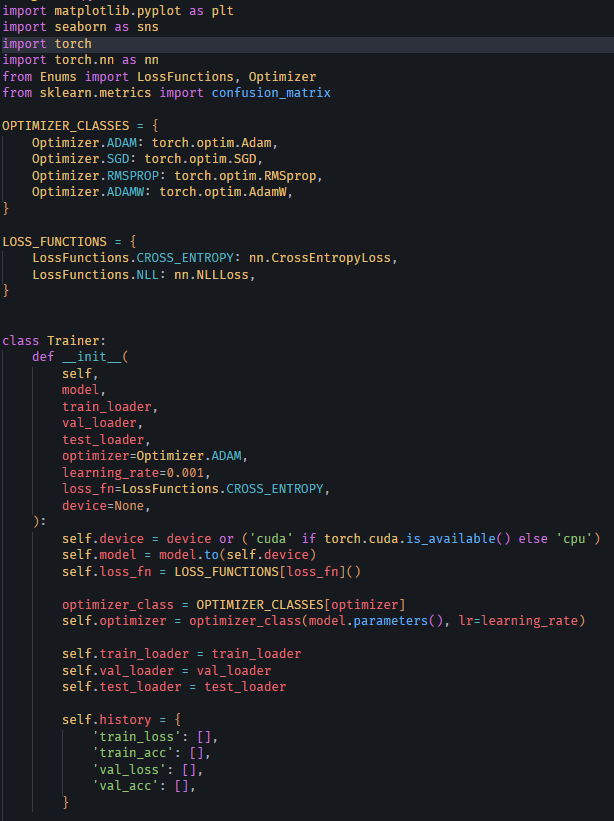
\includegraphics[width=0.85\linewidth]{3Lab/overleaf/images/Trainer_Class_1.png}
    \caption{Mokymo klasės kodas I dalis.}
    \label{fig:trainer_class_first}
\end{figure}

\begin{figure}[H]
    \centering
    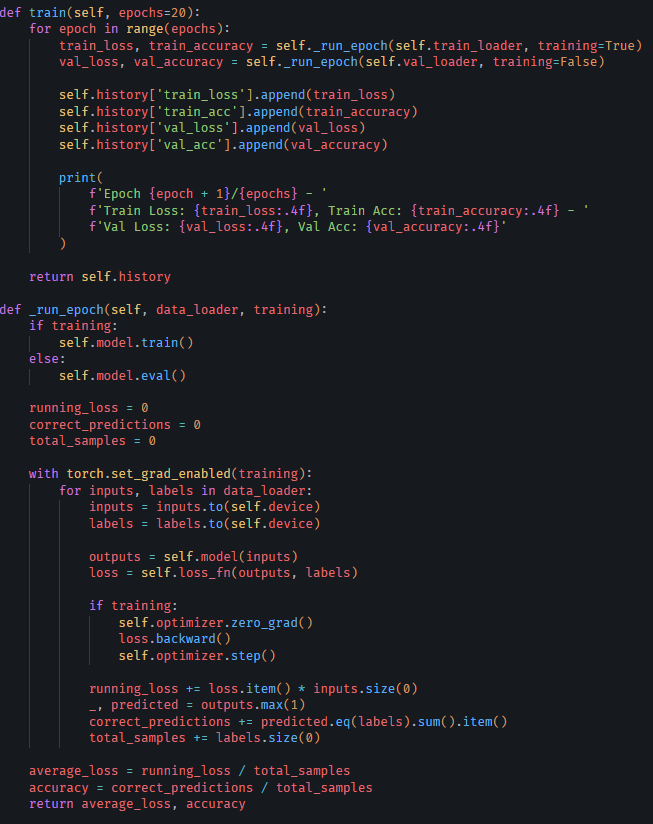
\includegraphics[width=0.85\linewidth]{3Lab/overleaf/images/Trainer_Class_2.png}
    \caption{Mokymo klasės kodas II dalis.}
    \label{fig:trainer_class_2}
\end{figure}

\begin{figure}[H]
    \centering
    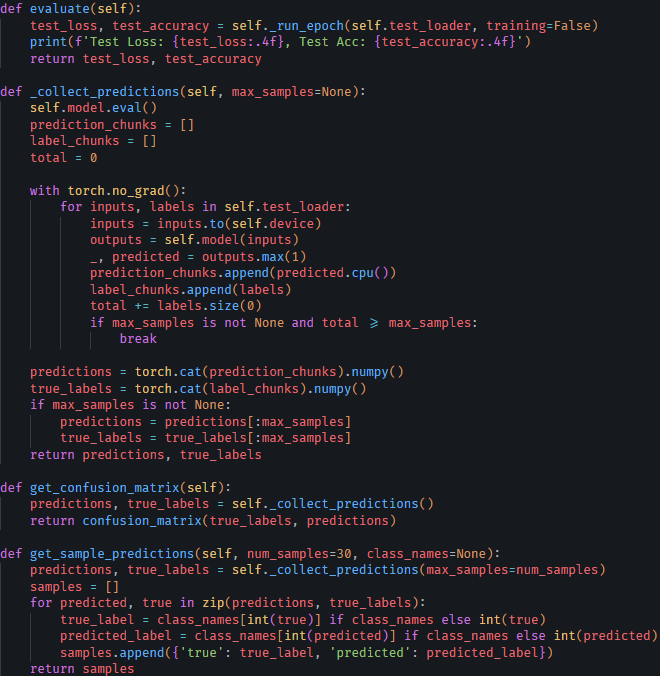
\includegraphics[width=0.85\linewidth]{3Lab/overleaf/images/Trainer_Class_3.png}
    \caption{Mokymo klasės kodas III dalis.}
    \label{fig:trainer_class_3}
\end{figure}

\begin{figure}[H]
    \centering
    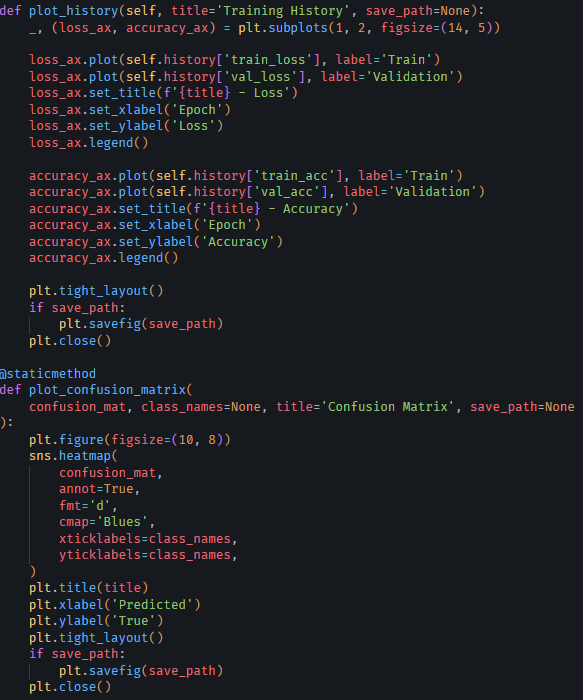
\includegraphics[width=0.85\linewidth]{3Lab/overleaf/images/Trainer_Class_4.png}
    \caption{Mokymo klasės kodas IV dalis.}
    \label{fig:trainer_class_4}
\end{figure}

\begin{figure}[H]
    \centering
    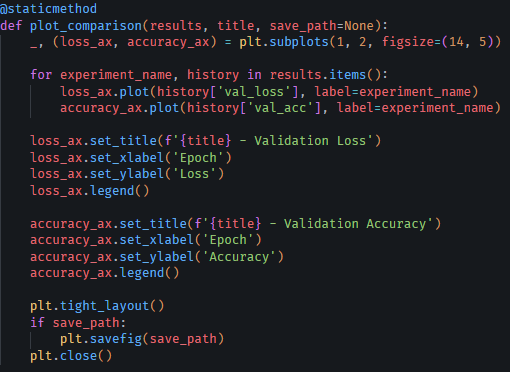
\includegraphics[width=0.85\linewidth]{3Lab/overleaf/images/Trainer_Class_5.png}
    \caption{Mokymo klasės kodas V dalis.}
    \label{fig:trainer_class_last}
\end{figure}

Klasės atsakomybės:
\begin{itemize}
    \item \texttt{train(epochs)} – kviečia \texttt{\_run\_epoch} mokymo ir validavimo aibėms kiekvienoje epochoje; kaupia keturių metrikų istoriją (\texttt{train\_loss}, \texttt{train\_acc}, \texttt{val\_loss}, \texttt{val\_acc}).
    \item \texttt{\_run\_epoch} – vienos epochos ciklas. Mokymo režime perjungia \texttt{model.train()}, validavimo / testavimo – \texttt{model.eval()}. Pagrindiniai žingsniai: paskaičiuoti \texttt{loss}, atlikti \texttt{loss.backward()} ir \texttt{optimizer.step()}, sumuoti tikslumą.
    \item \texttt{evaluate} – paleidžia tinklą ant testavimo aibės be gradiento skaičiavimo (\texttt{torch.no\_grad}).
    \item \texttt{get\_confusion\_matrix} – surenka spėjimus visam testavimo \texttt{DataLoader}'iui ir kviečia \texttt{sklearn.metrics.confusion\_matrix}.
    \item \texttt{get\_sample\_predictions(num\_samples)} – grąžina pirmųjų \texttt{num\_samples} testinių įrašų spėjimus su tikromis klasėmis (panaudota $30$ pavyzdžių sekcijoje).
    \item \texttt{plot\_history}, \texttt{plot\_confusion\_matrix}, \texttt{plot\_comparison} – \texttt{matplotlib} ir \texttt{seaborn} grafikai eksperimentų vizualizavimui.
\end{itemize}

Mokymo metu naudojamas:
\begin{itemize}
    \item \textbf{Paklaidos funkcija} \texttt{nn.CrossEntropyLoss} – matuoja, kaip toli tinklo \textit{logits} nuo tikrų klasių (žemo tikslumo prognozės baudžiamos labiau).
    \item \textbf{Optimizatorius} – konfigūruojamas per \texttt{Optimizer} enumeraciją (\textit{Adam} pagal nutylėjimą).
    \item \textbf{Tikslumo skaičiavimas} – \texttt{outputs.max(1)} grąžina kiekvienai eilutei didžiausios \textit{logit} reikšmės indeksą; lyginama su tikra klase.
\end{itemize}

Klasės architektūra ir mokymo ciklas suprogramuoti autoriaus. \texttt{matplotlib} / \texttt{seaborn} grafikų braižymo metodų \texttt{plot\_history}, \texttt{plot\_confusion\_matrix} ir \texttt{plot\_comparison} kvietimo šablonams panaudotos Claude pasiūlytos paruoštos formos, kurios vėliau pritaikytos prie projekto poreikių.

\subsection{Eksperimentų orkestracija (\texttt{main.py})}
\label{subsec:main_orchestration}

Failas \texttt{main.py} sujungia visas pirmiau aprašytas klases į vientisą eksperimentų vykdymo procesą: užkrauna duomenis, paleidžia penkis tyrimus, paskaičiuoja kiekvieno modelio metrikas ir parenka geriausią modelį testavimui (žr.~\ref{fig:main_first} – \ref{ref:main_last} pav.).

\begin{figure}[H]
    \centering
    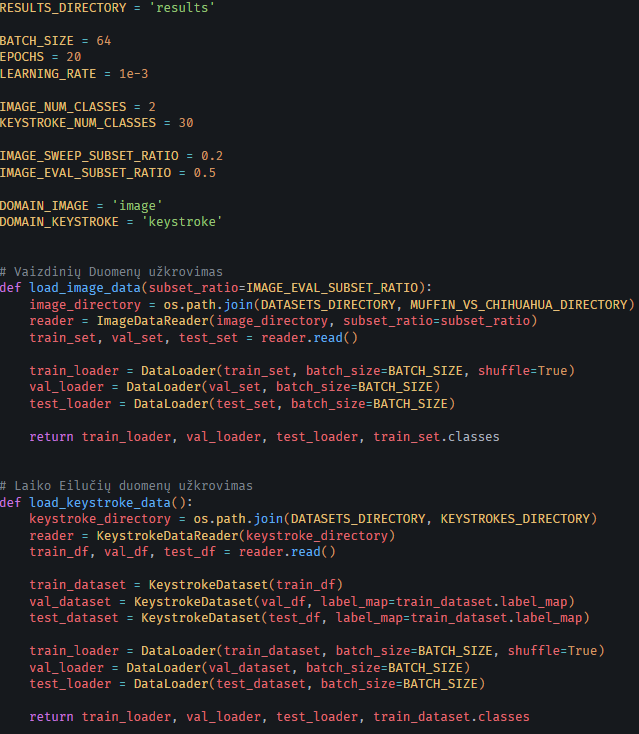
\includegraphics[width=0.85\linewidth]{3Lab/overleaf/images/main_1.png}
    \caption{Eksperimentų orkestracijos kodas I dalis.}
    \label{fig:main_first}
\end{figure}

\begin{figure}[H]
    \centering
    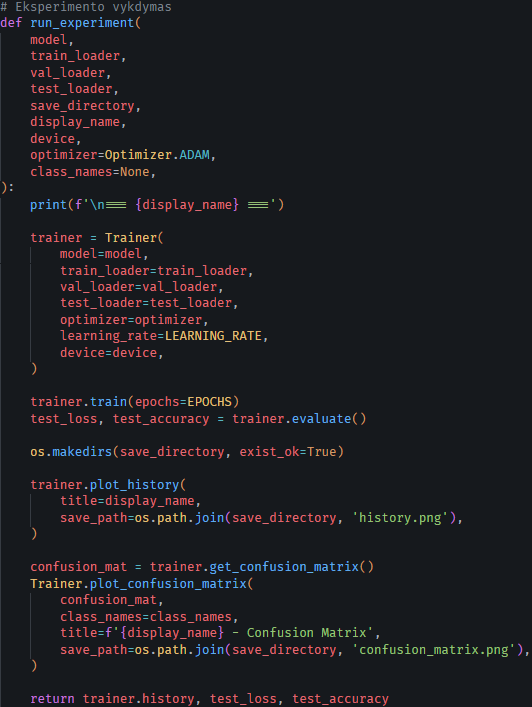
\includegraphics[width=0.85\linewidth]{3Lab/overleaf/images/main_2.png}
    \caption{Eksperimentų orkestracijos kodas II dalis.}
    \label{fig:main_second}
\end{figure}

\begin{figure}[H]
    \centering
    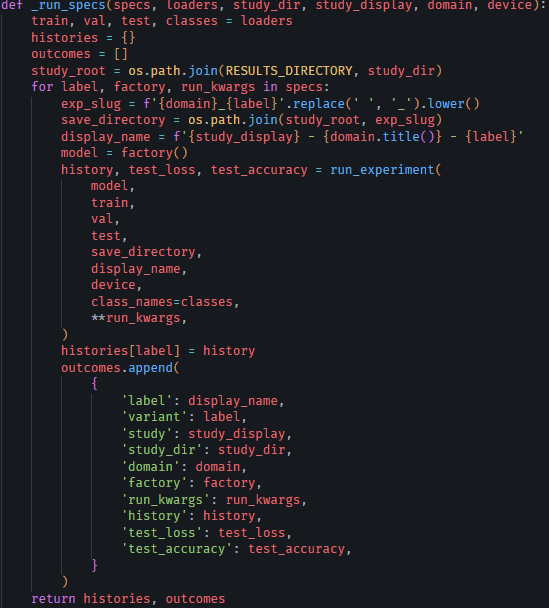
\includegraphics[width=0.85\linewidth]{3Lab/overleaf/images/main_3.png}
    \caption{Eksperimentų orkestracijos kodas III dalis.}
    \label{fig:main_third}
\end{figure}

\begin{figure}[H]
    \centering
    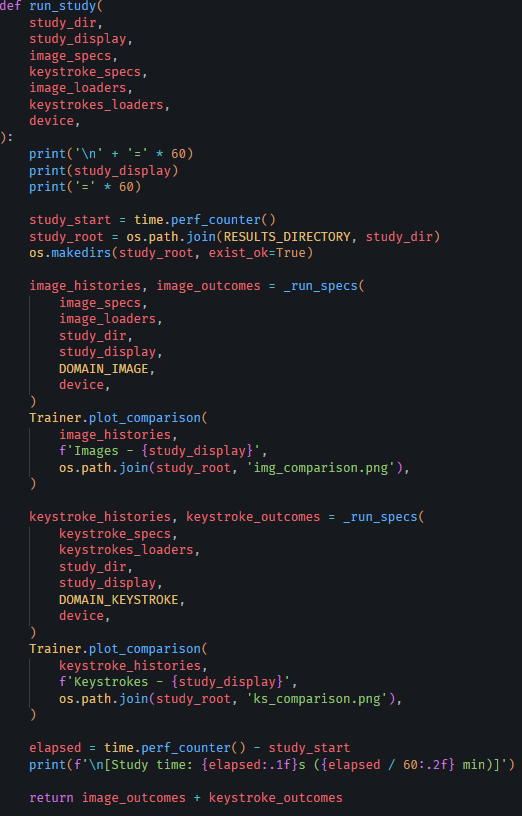
\includegraphics[width=0.85\linewidth]{3Lab/overleaf/images/main_4.png}
    \caption{Eksperimentų orkestracijos kodas IV dalis.}
    \label{fig:main_fourth}
\end{figure}

\begin{figure}[H]
    \centering
    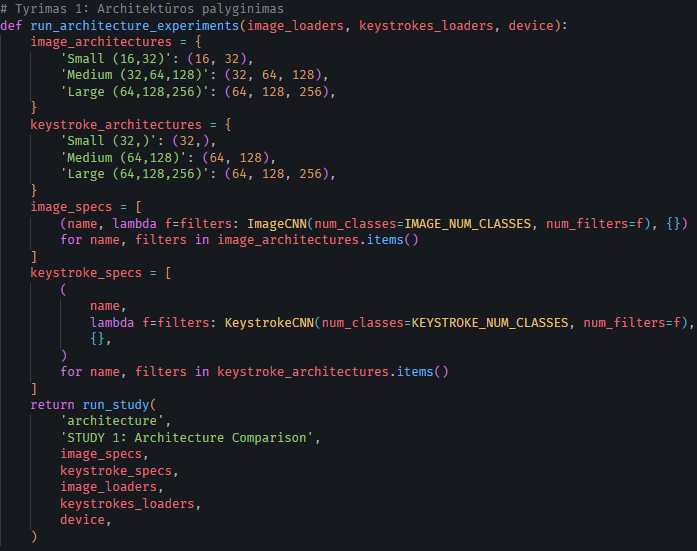
\includegraphics[width=0.85\linewidth]{3Lab/overleaf/images/main_5.png}
    \caption{Eksperimentų orkestracijos kodas V dalis.}
    \label{fig:main_fifth}
\end{figure}

\begin{figure}[H]
    \centering
    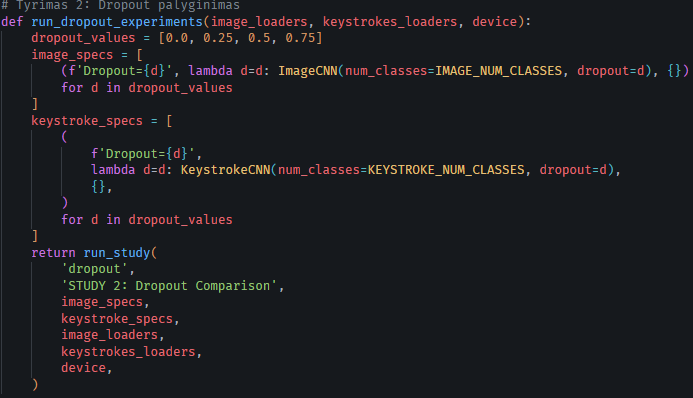
\includegraphics[width=0.85\linewidth]{3Lab/overleaf/images/main_6.png}
    \caption{Eksperimentų orkestracijos kodas VI dalis.}
    \label{fig:main_sixth}
\end{figure}

\begin{figure}[H]
    \centering
    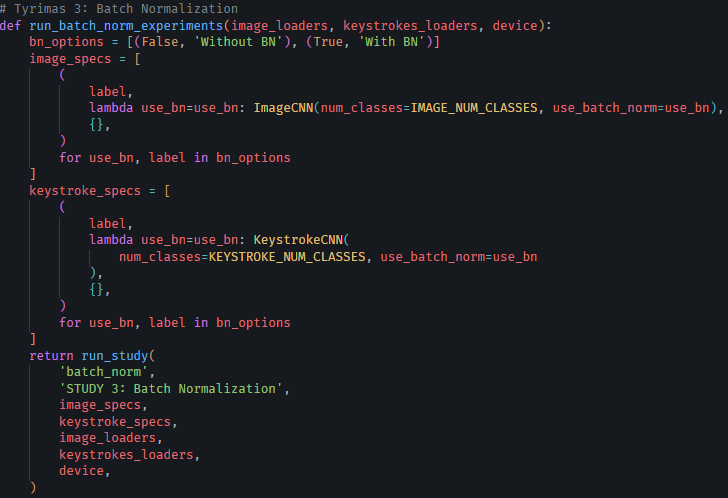
\includegraphics[width=0.85\linewidth]{3Lab/overleaf/images/main_7.png}
    \caption{Eksperimentų orkestracijos kodas VII dalis.}
    \label{fig:main_seventh}
\end{figure}

\begin{figure}[H]
    \centering
    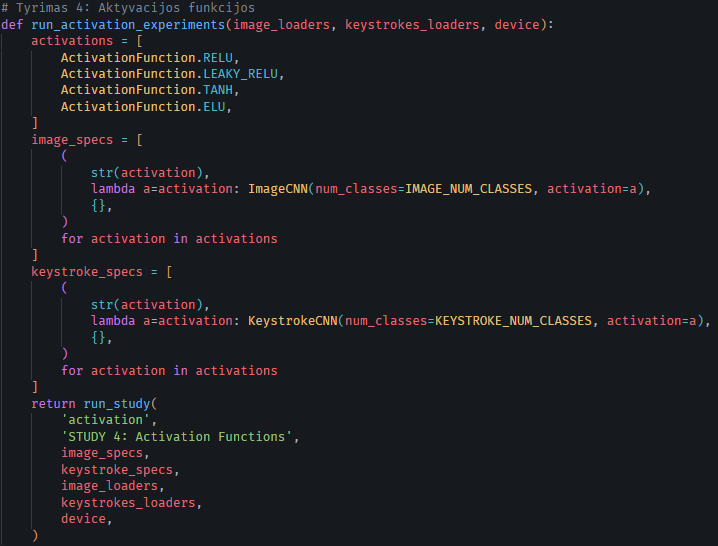
\includegraphics[width=0.85\linewidth]{3Lab/overleaf/images/main_8.png}
    \caption{Eksperimentų orkestracijos kodas VIII dalis.}
    \label{fig:main_eighth}
\end{figure}

\begin{figure}[H]
    \centering
    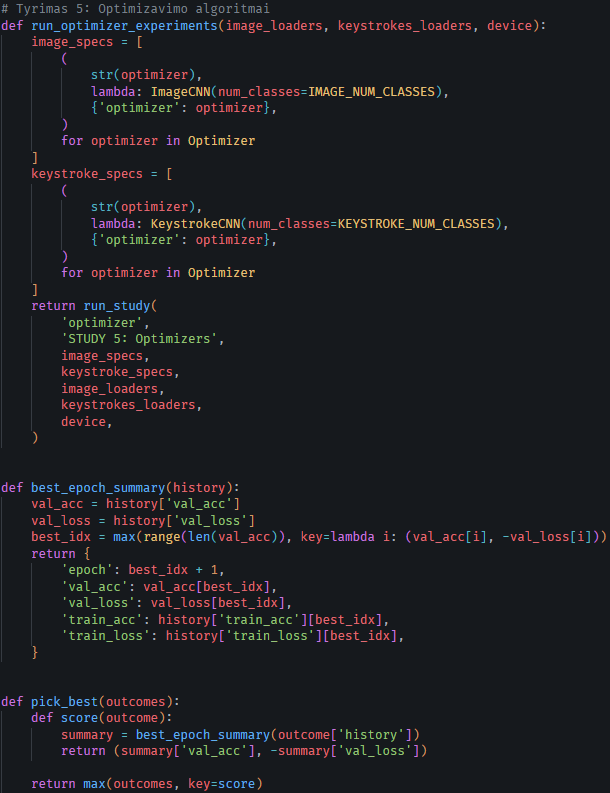
\includegraphics[width=0.85\linewidth]{3Lab/overleaf/images/main_9.png}
    \caption{Eksperimentų orkestracijos kodas IX dalis.}
    \label{fig:main_ninth}
\end{figure}

\begin{figure}[H]
    \centering
    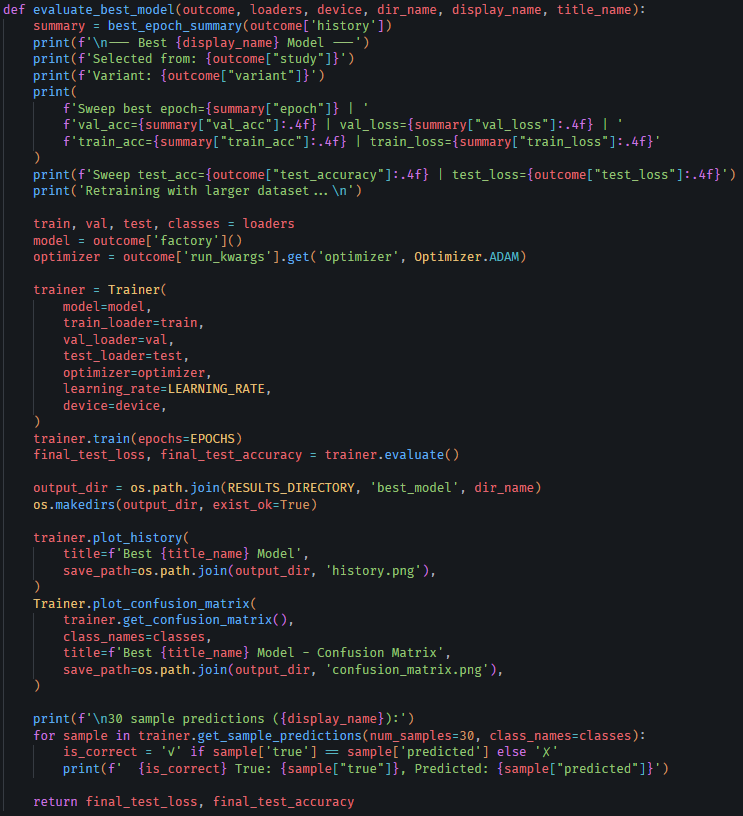
\includegraphics[width=0.85\linewidth]{3Lab/overleaf/images/main_10.png}
    \caption{Eksperimentų orkestracijos kodas X dalis.}
    \label{fig:main_10}
\end{figure}

\begin{figure}[H]
    \centering
    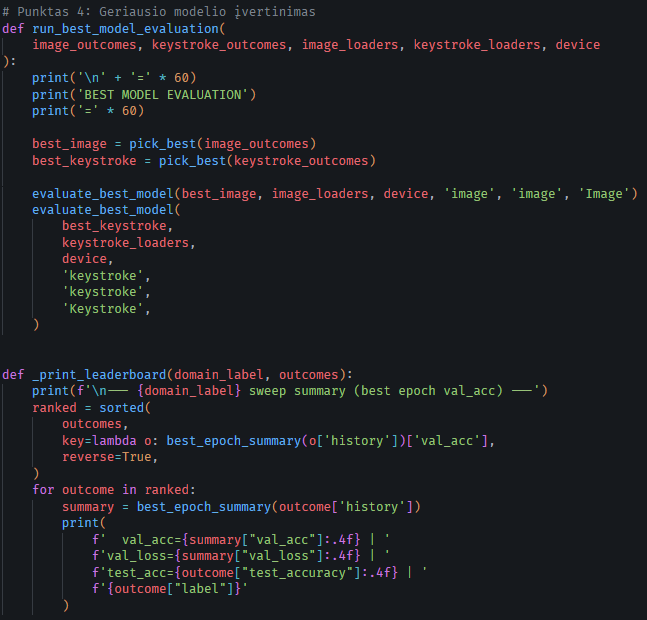
\includegraphics[width=0.85\linewidth]{3Lab/overleaf/images/main_11.png}
    \caption{Eksperimentų orkestracijos kodas XI dalis.}
    \label{fig:main_last}
\end{figure}

Pagrindinės funkcijos:
\begin{itemize}
    \item \texttt{load\_image\_data} ir \texttt{load\_keystroke\_data} – sukuria \texttt{DataLoader} objektus visoms trims aibėms; vaizdams perduoda \texttt{subset\_ratio} parametrą.
    \item \texttt{run\_experiment} – sukuria \texttt{Trainer}, paleidžia mokymą $20$ epochų, įvertina ant testavimo aibės ir išsaugo istorijos bei klasifikavimo matricos paveikslėlius.
    \item \texttt{run\_study} – paleidžia visus eksperimentus, priklausančius vienam tyrimui, ir sugeneruoja palyginimo grafiką (\textit{val\_loss} ir \textit{val\_acc} priklausomybės nuo epochos).
    \item \texttt{run\_architecture\_experiments}, \texttt{run\_dropout\_experiments}, \texttt{run\_batch\_norm\_experiments}, \texttt{run\_activation\_experiments}, \texttt{run\_optimizer\_experiments} – penki tyrimai, atitinkantys užduoties reikalavimus (žr.~\ref{sec:tyrimo_rezultatai} sk.).
    \item \texttt{pick\_best} – iš visų $17$ eksperimentų variantų atrenka geriausią pagal didžiausią validavimo tikslumą ir mažiausią validavimo paklaidą (lygiosioms taikomas leksikografinis kriterijus).
    \item \texttt{evaluate\_best\_model} – iš naujo apmoko geriausią konfigūraciją su didesniu vaizdų poaibiu (\texttt{subset\_ratio}~$=0{,}5$), išsaugo galutines istorijos ir klasifikavimo matricos vizualizacijas, atspausdina $30$ testinių pavyzdžių spėjimus.
\end{itemize}

